\section{\texorpdfstring{\centering CAPÍTULO II APLICACIÓN PRÁCTICA: CLASIFICACIÓN DE COBERTURA AGRÍCOLA}{CAPÍTULO II APLICACIÓN PRÁCTICA: CLASIFICACIÓN DE COBERTURA AGRÍCOLA}}

La clasificación de cobertura agrícola es una tarea fundamental en la agricultura de precisión, esto porque permite identificar y mapear las áreas cultivadas y no cultivadas en determinada región, incluso poder diferenciarlas de aquellas donde solo hay vegetación natural. Esta información es crucial para la toma de decisiones informadas en la gestión agrícola, optimización del uso de recursos y monitoreo del crecimiento de los cultivos. En este capítulo, se presenta una aplicación práctica de generación de un modelo de clasificación supervisada de cobertura agrícola utilizando unos de los datasets de información espacial más recientes y de libre acceso como lo es AlphaEarth Foundations.

\subsection{Flujo de trabajo}

A continuación se muestra el flujo de trabajo seguido para la generación del modelo de clasificación supervisada de cobertura agrícola:
\begin{figure}[H]
  \centering
  \includegraphics[trim=0.8cm 1cm 0.8cm 0.7cm, clip, width=0.98\linewidth]{assets/flujo.png}
  \caption{\centering Diagrama de flujo que describe el proceso de generación y uso del modelo de clasificación supervisada de cobertura agrícola.}
  \label{fig:flujo-trabajo}
\end{figure}

\newpage

\subsection{Materiales}

Las herramientas que se utilizarán para la generación y uso del modelo de clasificación supervisada de cobertura agrícola representan un poderoso conjunto de recursos para el análisis geoespacial que combina tecnología, datos, algoritmos avanzados e inteligencia artificial. Estas herramientas permiten a los usuarios procesar, analizar e interpretar grandes volúmenes de datos geoespaciales de manera eficiente y efectiva. 

\begin{itemize}
  \item \textbf{AlphaEarth Foundations}: Creado por Google DeepMind, AlphaEarth Foundations es un modelo de campos de embeddings (\textit{embedding field model} EFM) que combina datos geoespaciales de muchas diferentes fuentes y utiliza un algoritmo de aprendizaje automático para crear representaciones vectoriales (embeddings) de ubicaciones geográficas en todo el mundo. Estas representaciones vectoriales capturan características espaciales y temporales de las ubicaciones generando así una especie de "huella digital" para cada lugar en la Tierra. Estas representaciones vectoriales pueden ser utilizadas para una variedad de aplicaciones, incluyendo la clasificación de imágenes satelitales, la detección de cambios en el uso del suelo, la predicción de fenómenos naturales y la mejora de modelos climáticos. De manera simplificada, AlphaEarth Foundations es un dataset que proporciona información geoespacial rica y detallada es sus "bandas" que son son 64 en total, las cuales por sí solas no tienen un significado específico, ya que son representaciones matemáticas de características geoespaciales. Sin embargo, cuando se combinan y analizan en conjunto, estas bandas pueden proporcionar información valiosa sobre la superficie terrestre y sus cambios a lo largo del tiempo. \cite{Brown2025}
  \item \textbf{Google Earth Engine (GEE)}: Propiedad de Google, es una plataforma en la nube que permite a los usuarios analizar y visualizar grandes conjuntos de datos geoespaciales. Proporciona acceso a una vasta colección de imágenes satelitales y datos geoespaciales, junto con herramientas de procesamiento y análisis avanzadas. GEE es ampliamente utilizado en la investigación ambiental, la gestión de recursos naturales, la agricultura de precisión y otros campos relacionados con el análisis geoespacial. La plataforma permite a los usuarios realizar análisis complejos sin necesidad de descargar grandes volúmenes de datos, lo que facilita el trabajo con conjuntos de datos masivos. \cite{Pizarro2022}. Para el caso de estudio, esta plataforma se utiliza para la generación del modelo, pruebas y uso del mismo.
  \item \textbf{QGIS (Quantum Geographic Information System)}: Es un sistema de información geográfica (SIG) de código abierto que permite a los usuarios crear, editar, visualizar, analizar y publicar información geoespacial. QGIS es una herramienta poderosa y versátil que es ampliamente utilizada en diversas disciplinas, incluyendo la agricultura de precisión, la gestión ambiental, la planificación urbana y la investigación científica. QGIS ofrece una amplia gama de funcionalidades, incluyendo la capacidad de trabajar con múltiples formatos de datos geoespaciales, realizar análisis espaciales avanzados, crear mapas personalizados y automatizar tareas mediante scripts. La plataforma es altamente extensible a través de complementos (plugins) que permiten a los usuarios agregar funcionalidades específicas según sus necesidades. \cite{Cubillas2024}. Este software se utilizará para la generación de las etiquetas de entrenamiento que representan junto al al dataset de AlphaEarth Foundations, los datos de entrada para la generación del modelo de clasificación supervisada de cobertura agrícola.
  \item \textbf{Random Forest}: Es un algoritmo de aprendizaje automático supervisado que se utiliza para tareas de clasificación y regresión. Fue desarrollado por Leo Breiman y Adele Cutler en la década de 1990 y se basa en la idea de combinar múltiples árboles de decisión para mejorar la precisión y robustez del modelo. En lugar de construir un solo árbol de decisión, Random Forest crea un conjunto (o "bosque") de árboles de decisión independientes, cada uno entrenado en una muestra aleatoria del conjunto de datos original. Durante el proceso de entrenamiento, cada árbol toma decisiones basadas en diferentes subconjuntos de características y datos, lo que ayuda a reducir el sobreajuste y mejora la capacidad del modelo para generalizar a nuevos datos. Para la generación del modelo de clasificación supervisada de cobertura agrícola, se utiliza la implementación de Random Forest disponible en Google Earth Engine. \cite{BarbozaCastillo2022}
\end{itemize}

\newpage

\subsection{Metodología}

La metodología seguida para la clasificación supervisada de cobertura agrícola utilizando AlphaEarth Foundations y Google Earth Engine (GEE) se detalla a continuación, enfocando el área geográfica en el departamento de Lambayeque, Perú:

\begin{itemize}
  \item \textbf{Tipo de análisis}: Aplicado, cuantitativo, descriptivo y explicativo.
  \item \textbf{Unidad de análisis}: Pixel satelital (10 m x 10 m).
  \item \textbf{Periodo de estudio}: Enero 2020 - Diciembre 2024.
  \item \textbf{Área de estudio}: Modelo de clasificación de cobertura agrícola válido para el departamento de Lambayeque, Perú.
  \item \textbf{Justificación del área de estudio}: Lambayeque es una región costera con una importante actividad agrícola, caracterizada por una cobertura agrícola bien delimitada y homogénea, lo que facilita la generación y validación del modelo. Además, la diferenciación entre áreas agrícolas y vegetación natural es más clara en comparación con otras regiones del país como la Selva o la Sierra, donde la diversidad de cultivos y la presencia de vegetación natural pueden complicar el proceso de clasificación.
  \item \textbf{Fuentes de datos}: AlphaEarth Foundations y Google Earth Engine.
  \item \textbf{Software}: Google Earth Engine y QGIS.
  \item \textbf{Complementarios}: Google Maps, límites administrativos del Perú (INEI).
\end{itemize}

\begin{figure}[H]
  \centering
  \includegraphics[width=0.9\linewidth]{assets/mapaDeUbicacion.png}
  \caption{\centering Mapa de ubicación del departamento de Lambayeque, Perú, área de estudio para la clasificación de cobertura agrícola.}
  \label{fig:mapa-ubicacion}
\end{figure}

\subsection{Procedimiento}
De acuerdo al flujo de trabajo, la generación del modelo de clasificación supervisada de cobertura agrícola y posterior uso del mismo contempla la secuencia de pasos que inician con la generación de etiquetas de entrenamiento. AlphaEarth Foundations brinda 64 bandas que representan características geoespaciales, las cuales se toman como entrada para la generación de un dataset nuevo que describe las características de estas bandas para cada polígono de las etiquetas de entrenamiento, lo que posteriormente se utiliza para entrenar el modelo de clasificación.

\subsubsection{Etiquetas de entrenamiento}
Para la generación de etiquetas de entrenamiento, se generará un recurso vectorial en QGIS que contenga polígonos que, a modo de muestra, representen los diferentes tipos de cobertura agrícola presentes en el departamento de Lambayeque, así como áreas sin cobertura agrícola, como zonas urbanas, cuerpos de agua y vegetación natural. Estos polígonos deben ser lo más representativos y variados posibles para asegurar que el modelo pueda aprender a diferenciarlas, lo cual es importante dada la naturaleza estadística del algoritmo.

\begin{itemize}
  \item \textbf{Área de Interés (AOI)}: Para la delimitación del área de estudio, se utilizará un recurso vectorial con los límites departamentales de Lambayeque, el cual puede ser descargado desde el portal del INEI \cite{inei} mediante la capa de "Departamentos" actualizado al año 2023. Este recurso será útil tanto para la delimitación del área de entrenamiento del modelo como para la posterior aplicación del mismo, además, servirá para delimitar los polígonos de las etiquetas de entrenamiento. La elección del departamento de Lambayeque se justifica por ser una región con una importante actividad agrícola, productos como caña de azucar, paltos, arándanos, limones, etc, son cultivados en grandes extensiones y representan uno de los motores económicos de la región por su gran volumen de exportación.
  \item \textbf{Imagen de referencia}: Se utilizarán imágenes compuestas de Sentinel-2. Es importante que la generación de etiquetas de entrenamiento se realice con imágenes de la misma fecha de adquisición que las imágenes que se utilizarán para la clasificación, ya que las características espectrales de los cultivos pueden variar dependiendo de la etapa fenológica en la que se encuentren.
  \begin{itemize}
    \item Fecha de adquisición: 01-01-2024 - 02-01-2024.
    \item Fuente: Sentinel-2.
    \item Resolución espacial: 10 m.
    \item Bandas: B4 (Red), B3 (Green), B2 (Blue).
    \item Área de interés: Departamento de Lambayeque, Perú.
    \item Plataforma: Google Earth Engine.
  \end{itemize}

  A continuación se muestra el código en JavaScript utilizado en Google Earth Engine para la generación de la imagen de referencia:

  \begin{figure}[H]
  \centering
  \begin{minipage}{0.8\linewidth}
  \begin{minted}[frame=lines, linenos, breaklines, fontsize=\small]{javascript}
    var sentinel = ee.ImageCollection("COPERNICUS/S2_SR_HARMONIZED")
      .filterDate('2024-01-01', '2024-01-02')
      .filterBounds(aoiLambayeque);
  
    var visParamsSentinel = {
      bands: ['B4', 'B3', 'B2'],
      min: 0,
      max: 3000,
      gamma: 1.2
    };
  \end{minted}
  \end{minipage}
  \caption{\centering Código en JavaScript para la generación de la imagen de referencia en GEE. De la línea 1 a 4, se carga el dataset de Sentinel-2 y se filtra por fecha y área de interés, y de la línea 6 a 11, se definen los parámetros de visualización para la imagen.}
  \label{fig:codigo_modelo9}
\end{figure}

  \item \textbf{Generación de etiquetas}: Con la imagen de referencia descargada y en QGIS, se crearán polígonos que representen las diferentes clases de cobertura agrícola y no agrícola. Cada polígono debe ser etiquetado con la clase correspondiente, se utilizan 0 para áreas sin cobertura agrícola, 1 para área de cultivos. Es recomendable crear múltiples polígonos para cada clase para capturar la variabilidad dentro de cada categoría. La cantidad de polígonos serán de 150 por cada clase.

  A continuación, se muestra un ejemplo de las etiquetas de entrenamiento generadas en QGIS para el departamento de Lambayeque: 

\begin{figure}[H]
  \centering
  \begin{minipage}{0.45\textwidth}
    \centering
    \includegraphics[trim=1cm 1cm 1cm 1cm, clip, width=\linewidth]{assets/referencia.png}
    \caption*{(a) Imagen de referencia (Sentinel-2)}
  \end{minipage}\hfill
  \begin{minipage}{0.55\textwidth}
    \centering
    \includegraphics[trim=1cm 1cm 1cm 1cm, clip, width=\linewidth]{assets/etiquetado.png}
    \caption*{(b) Etiquetado de polígonos en QGIS}
  \end{minipage}
  \hfill
  \begin{minipage}{0.9\textwidth}
    \centering
    \includegraphics[trim=1cm 1cm 1cm 1cm, clip, width=\linewidth]{assets/poligonizacion.png}
    \caption*{(c) Muestra de polígonos realizados}
  \end{minipage}
  \caption{\centering Muestra del etiquetado de polígonos en QGIS para la generación del dataset  de entrenamiento en el departamento de Lambayeque, Perú. Nótese que en (a) se muestra la imagen de referencia utilizada, en (b) el proceso de etiquetado de polígonos y en (c) una muestra de los polígonos realizados.}
  \label{fig:etiquetas-lambayeque}
\end{figure}

\newpage
  \item \textbf{Exportación de etiquetas}: Una vez hechos y revisados los polígonos en QGIS, se exportan como un archivo shapefile (.shp), formato compatible con Google Earth Engine. Este archivo contendrá las coordenadas y las etiquetas de clase para cada polígono, que serán utilizadas en el siguiente paso para extraer las características de AlphaEarth Foundations.
  
  \begin{figure}[H]
  \centering
  \begin{minipage}{1\textwidth}
    \centering
    \includegraphics[trim=1cm 1cm 9.25cm 4cm, clip, width=\linewidth]{assets/subido.png}
    \caption*{Recurso shapefile subido en GEE}
  \end{minipage}
  \caption{\centering Subida del archivo shapefile con las etiquetas de entrenamiento a Google Earth Engine.}
  \label{fig:proceso_subida}
\end{figure}
\end{itemize}

\subsubsection{Generación del dataset de entrenamiento}

Una vez subidos los recursos necesarios para la generación del modelo de clasificación supervisada de cobertura agrícola, se procede a la generación del recurso necesario que describe las características de las 64 bandas de AlphaEarth Foundations para cada polígono de las etiquetas de entrenamiento, este recurso alojado en el ambiente de desarollo de Google Earth Engine, es un \textit{FeatureCollection} que contiene las características de las mencionadas 64 bandas. 

\begin{figure}[H]
  \centering
  \begin{minipage}{0.8\linewidth}
\begin{minted}[frame=lines, linenos, breaklines, fontsize=\small]{javascript}
var aoiLambayeque = ee.FeatureCollection("projects/test-hsluis4326/assets/aoiLambayeque"),
    etiquetas = ee.FeatureCollection("projects/test-hsluis4326/assets/etiquetas");
\end{minted}
  \end{minipage}
  \caption{\centering Código en JavaScript para la importación de los recursos necesarios en GEE. La ubicación de los recursos varían dependiendo del usuario y proyecto GEE.}
  \label{fig:codigo_modelo}
\end{figure}
\newpage
A continuación, se muestra el código en JavaScript utilizado en Google Earth Engine para la generación del dataset de entrenamiento, nótese que se utiliza el método \texttt{sampleRegions()} para extraer las características para cada polígono de las etiquetas de entrenamiento.

\begin{figure}[H]
  \centering
  \begin{minipage}{0.8\linewidth}
\begin{minted}[frame=lines, linenos, breaklines, fontsize=\small]{javascript}
var dataset = ee.ImageCollection("GOOGLE/SATELLITE_EMBEDDING/V1/ANNUAL")
  .filterDate('2024-01-01', '2024-01-02')
  .filterBounds(aoiLambayeque);

var imageAlpha = dataset.mosaic().clip(aoiLambayeque);

var samples = imageAlpha.sampleRegions({
  collection: etiquetas,
  properties: ['clase'],
  scale: 20,
});
\end{minted}
  \end{minipage}
  \caption{\centering Código en JavaScript para la generación del dataset de entrenamiento en GEE. De la línea 1 a 3, se carga el dataset de AlphaEarth Foundations, de la línea 5 a 7, se genera una imagen mosaico y se recorta al área de interés, y de la línea 9 a 13, se genera el dataset de entrenamiento utilizando las etiquetas de entrenamiento. Obs: se utiliza una escala de 20 metros para la extracción de las características por su alta carga computacional.}
  \label{fig:codigo_modelo_2}
\end{figure}

\subsubsection{Generación del modelo de clasificación supervisada}

Con el dataset de entrenamiento generado, se procede a la creación del modelo de clasificación supervisada utilizando el algoritmo de Random Forest disponible en Google Earth Engine. A continuación, se muestra el código en JavaScript utilizado para la generación del modelo:

\begin{figure}[H]
  \centering
  \begin{minipage}{0.8\linewidth}
\begin{minted}[frame=lines, linenos, breaklines, fontsize=\small]{javascript}
var classifier = ee.Classifier.smileRandomForest(200).train({
  features: samples,
  classProperty: 'clase',
  inputProperties: imageAlpha.bandNames()
});
\end{minted}
  \end{minipage}
  \caption{\centering Código en JavaScript para la generación del modelo de clasificación supervisada en GEE. En este caso, se utiliza 200 árboles de decisión para la creación del modelo. Nótese, además, que se especifica la propiedad de clase y las bandas de entrada.}
  \label{fig:codigo_modelo_3}
\end{figure}

\subsubsection{Aplicación del modelo de clasificación supervisada}

El modelo de clasificación supervisada generada se aplica sobre el mismo dataset de AlphaEarth Foundations utilizado para la generación del modelo, pero esta vez, para todo el departamento de Lambayeque. Una vez procesada la imagen, se visualizan los resultados obtenidos en un mapa de clasificación, donde cada píxel resulta en una máscara que indica la clase asignada por el modelo, 0 para áreas sin cobertura agrícola y 1 para áreas con cobertura agrícola.
\begin{figure}[H]
  \centering
  \begin{minipage}{0.8\linewidth}
\begin{minted}[frame=lines, linenos, breaklines, fontsize=\small]{javascript}
var classified = imageAlpha.classify(classifier);

Map.addLayer(classified, {min:0, max:1, palette:['red','green']}, 'Clasificación');
\end{minted}
  \end{minipage}
  \caption{\centering Código en JavaScript para la aplicación del modelo de clasificación supervisada en GEE. La generación de la imagen clasificada se realiza mediante el método \texttt{classify()} y la visualización de la misma en el lienzo mediante \texttt{Map.addLayer()} con una paleta de colores tal que las áreas sin cobertura agrícola se muestran en rojo y las áreas con cobertura agrícola en verde.}
  \label{fig:codigo_modelo_4}
\end{figure}

\subsection{Resultados}

El producto obtenido tras la aplicación del modelo de clasificación supervisada de cobertura agrícola es una capa ráster que muestra la clasificación de cada píxel en el área de estudio, como se explicó en los fundamentos teóricos, la salida es la representación de una máscara binaria (matriz) donde cada píxel es clasificado en una de las dos categorías: áreas con cobertura agrícola (1) y áreas sin cobertura agrícola (0). A continuación, se muestra el mapa de clasificación obtenido para el departamento de Lambayeque sobre la imagen de referencia, entrenada con etiquetas y generada con AlphaEarth Foundations:

\begin{figure}[H]
  \centering
  \includegraphics[trim=1cm 1cm 1cm 1cm, clip, width=1\linewidth]{assets/mapaClasificacion.png}
  \caption{\centering Mapa de clasificación de cobertura agrícola obtenido para el departamento de Lambayeque, Perú, utilizando el modelo de clasificación supervisada generado con AlphaEarth Foundations y Google Earth Engine. En verde se muestran las áreas con cobertura agrícola y en rojo las áreas sin cobertura agrícola.}
  \label{fig:mapa-clasificacion}
\end{figure}

\subsection{Validación del modelo de clasificación supervisada}

Para la validación de la clasificación de cobertura agrícola mediante el modelo de Random Forest, se utilizan diversas métricas que permiten evaluar la precisión y confiabilidad del modelo aprovechando la naturaleza binaria de la clasificación. Los métodos de validación surgen a partir de la segmentación del dataset de entrenamiento en dos subconjuntos: uno para el entrenamiento del modelo (70\% de los datos) y otro para la validación (30\% de los datos). Esta división asegura que el modelo se evalúe con datos que no ha visto durante el entrenamiento, proporcionando una medida más realista de su rendimiento, posteriormente con el modelo ya validado y con métricas satisfactorias, se reentrena el modelo con el 100\% de los datos para su uso en producción. Se puede observar a continuación el código que genera la segmentación de los datos de entrenamiento y que servirán para la validación del mismo.  Finalmente, se entrena el modelo utilizando solo las muestras de entrenamiento y se imprimen en la consola las cantidades de muestras totales, de entrenamiento y de validación.

\begin{figure}[H]
  \centering
  \begin{minipage}{0.8\linewidth}
\begin{minted}[frame=lines, linenos, breaklines, fontsize=\small]{javascript}
var withRandom = samples.randomColumn('random');
var split = 0.7;
var trainingSamples = withRandom.filter(ee.Filter.lt('random', split));
var validationSamples = withRandom.filter(ee.Filter.gte('random', split));

var classifier = ee.Classifier.smileRandomForest(200).train({
  features: trainingSamples,
  classProperty: 'clase',
  inputProperties: imageAlpha.bandNames()
});

print('Total de muestras:', samples.size());
print('Muestras de entrenamiento:', trainingSamples.size());
print('Muestras de validación:', validationSamples.size());

\end{minted}
  \end{minipage}
  \caption{\centering Código en JavaScript para la segmentación del dataset de entrenamiento y generación del modelo de clasificación supervisada en GEE. Se utiliza el método \texttt{randomColumn()} para asignar un valor aleatorio a cada muestra, luego se filtran las muestras en dos subconjuntos: uno para entrenamiento (70\%) y otro para validación (30\%).}
  \label{fig:codigo_modelo_6}
\end{figure}

 Considérese que los valores reales corresponden a una escala de 20 metros por píxel lo que reduce la carga computacional, valores más bajos en escala generan más muestras y mejor precisión espacial, pero a costa de mayor tiempo de procesamiento. La salida de la consola de Google Earth Engine tras la ejecución del código anterior es la siguiente:

\begin{figure}[H]
  \centering
  \begin{minipage}{0.8\linewidth}
    \begin{minted}[frame=lines, linenos, breaklines, fontsize=\small]{bash}
      Total de muestras:
      51321
      Muestras de entrenamiento:
      35821
      Muestras de validación:
      15500
    \end{minted}
  \end{minipage}
  \caption{\centering Salida de la consola de Google Earth Engine tras la ejecución del código para la segmentación del dataset de entrenamiento y generación del modelo de clasificación supervisada, los valores corresponden a la cantidad de píxeles muestreados (51,321), de los cuales 35,821 se utilizan para el entrenamiento del modelo y 15,500 para la validación del mismo.}
  \label{fig:consola-gee}
\end{figure}
\newpage
\subsubsection{Matriz de confusión}

La matriz de confusión es una herramienta fundamental para evaluar el rendimiento de un modelo de clasificación. En este caso, se utiliza para comparar las predicciones del modelo con las etiquetas reales de un conjunto de datos de validación independiente. A continuación se muestra el proceso de obtención de la matriz de confusión, resultado e interpretación:

\begin{figure}[H]
  \centering
  \begin{minipage}{0.8\linewidth}
\begin{minted}[frame=lines, linenos, breaklines, fontsize=\small]{javascript}
var validation = validationSamples.classify(classifier);

var confusionMatrix = validation.errorMatrix('clase', 'classification');
print('Matriz de Confusión:', confusionMatrix);
\end{minted}
  \end{minipage}
  \caption{\centering Código en JavaScript para la obtención de la matriz de confusión en GEE. Se utiliza el método \texttt{errorMatrix()} para comparar las etiquetas reales con las predicciones del modelo.}
  \label{fig:codigo_modelo_5}
\end{figure}

Con la comparación entre las etiquetas reales y las predicciones del modelo, se obtiene la siguiente matriz de confusión:

\begin{table}[H]
\centering
\begin{tabular}{ccc}
\textbf{} & \textbf{Predicción: Cultivo} & \textbf{Predicción: No Cultivo} \\
\hline
\textbf{Clase: Cultivo} & 9481 & 4 \\
\textbf{Clase: No Cultivo} & 14 & 6001 \\
\hline
\end{tabular}
\caption{\centering Matriz de confusión obtenida para la validación del modelo de clasificación supervisada de cobertura agrícola.}
\label{tab:matriz-confusion}
\end{table}

Como se observa en la tabla \ref{tab:matriz-confusion}, la matriz de confusión muestra que el modelo ha clasificado correctamente 9,481 píxeles como ``Cultivo'' y 6,001 píxeles como ``No Cultivo''. Sin embargo, también ha cometido algunos errores, clasificando incorrectamente 4 píxeles como ``No Cultivo'' cuando en realidad son ``Cultivo'' (falsos negativos) y 14 píxeles como ``Cultivo'' cuando en realidad son ``No Cultivo'' (falsos positivos), sin embargo, estos errores son mínimos en comparación con la cantidad total de muestras, lo que indica un buen rendimiento del modelo. 

\subsubsection{Precisión General del modelo (overall accuracy)}

A partir de la matriz de confusión, se pueden calcular diversas métricas de precisión que proporcionan una evaluación cuantitativa del rendimiento del modelo. Esta métrica es especialmente aplicable en este caso ya que las etiquetas de entrenamiento están balanceadas, es decir, tal como se indicó anteriormente, se generaron 150 polígonos para cada clase (cultivo y no cultivo), lo que resulta en un conjunto de datos de entrenamiento equilibrado. El cálulo de la precisión general puede ser calculado mediante:
\[\text{Precisión General} = \frac{TP + TN}{TP + TN + FP + FN}\]
Donde:


\(TP\) (True Positives): Verdaderos positivos, clasificación correcta de ``Cultivo''.\\
\(TN\) (True Negatives): Verdaderos negativos, clasificación correcta de ``No Cultivo''.\\
\(FP\) (False Positives): Falsos positivos, clasificación incorrecta de ``Cultivo''.\\
\(FN\) (False Negatives): Falsos negativos, clasificación incorrecta de ``No Cultivo''.

\newpage

A continuación, se muestra la obtención de la precisión del modelo y su resultado:

\begin{figure}[H]
  \centering
  \begin{minipage}{0.8\linewidth}
\begin{minted}[frame=lines, linenos, breaklines, fontsize=\small]{javascript}
var overallAccuracy = confusionMatrix.accuracy();
print('Precisión general del modelo:', overallAccuracy);
\end{minted}
  \end{minipage}
  \caption{\centering Código en JavaScript para calcular la precisión general (overall accuracy) del modelo de clasificación supervisada en GEE a partir de la matriz de confusión.}
  \label{fig:codigo_modelo_7}
\end{figure}

La salida de la consola de Google Earth Engine tras la ejecución del código anterior es la siguiente:

\begin{figure}[H]
  \centering
  \begin{minipage}{0.8\linewidth}
    \begin{minted}[frame=lines, linenos, breaklines, fontsize=\small]{bash}
      Precisión Global (%):
      99.88387096774194
    \end{minted}
  \end{minipage}
  \caption{\centering Salida de la consola de Google Earth Engine tras la ejecución del código para calcular la precisión general del modelo de clasificación supervisada.}
  \label{fig:consola-gee-precision}
\end{figure}

Como se observa en la figura \ref{fig:consola-gee-precision}, la precisión general del modelo es del 99.88\%, lo que indica que el modelo ha clasificado correctamente el 99.88\% de las muestras de validación. Esta alta precisión sugiere que el modelo es muy efectivo para distinguir entre áreas con y sin cobertura agrícola en el área de estudio.

\subsubsection{Métricas de área calculada}

Además de la precisión general, se presentan los valores calculados de área general del departamento de Lambayeque, área clasificada como cobertura agrícola y área clasificada como sin cobertura agrícola, así como el porcentaje que representa cada una de estas áreas con respecto al total del departamento. Estos valores son importantes para entender la distribución espacial de la cobertura agrícola en la región y pueden ser útiles para la toma de decisiones en la gestión agrícola y planificación territorial.

\begin{table}[H]
\centering
\begin{tabular}{l|c}
\textbf{Estadística} & \textbf{Valor} \\
\hline
Área total (hectáreas) & 1,467,943.73 \\
Área agrícola (hectáreas) & 83,381.34 \\
Porcentaje de cobertura agrícola (\%) & 5.68 \\
Porcentaje de cobertura no agrícola (\%) & 94.32 \\
\end{tabular}
\caption{\centering Estadísticas de área calculadas para el departamento de Lambayeque.}
\label{tab:estadisticas-area}
\end{table}

\begin{figure}[H]
\centering
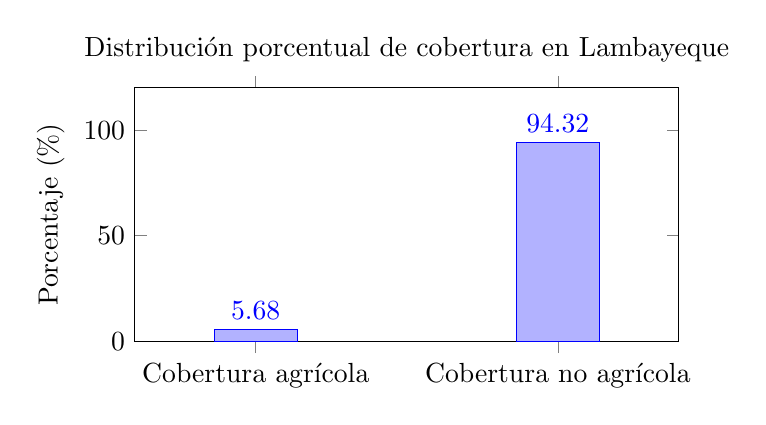
\begin{tikzpicture}
\begin{axis}[
  ybar,
  bar width=30pt,
  width=0.7\textwidth,
  height=4.8cm,
  ymin=0, ymax=120,
  ylabel={Porcentaje (\%)},
  symbolic x coords={Cobertura agrícola, Cobertura no agrícola},
  xtick=data,
  nodes near coords,
  nodes near coords align={vertical},
  enlarge x limits=0.4,
  title={Distribución porcentual de cobertura en Lambayeque}
]
\addplot coordinates {(Cobertura agrícola,5.68) (Cobertura no agrícola,94.32)};
\end{axis}
\end{tikzpicture}
\caption{\centering Gráfico de barras con la distribución porcentual de cobertura agrícola y no agrícola en Lambayeque.}
\label{fig:barra-cobertura}
\end{figure}

\subsection{Análisis y discusión de resultados}

Los resultados obtenidos en la clasificación de cobertura agrícola para el departamento de Lambayeque utilizando el modelo de Random Forest entrenado con AlphaEarth Foundations y Google Earth Engine son altamente satisfactorios. La precisión general del modelo, que alcanza un 99.88\%, indica que el modelo es extremadamente efectivo para distinguir entre áreas con y sin cobertura agrícola en la región. Esta alta precisión es un indicativo claro de que las características extraídas de AlphaEarth Foundations son adecuadas para esta tarea específica de clasificación. 

\subsubsection{Clasificación en áreas cubiertas por nubes}

Un aspecto importante a considerar en la clasificación de imágenes satelitales es la presencia de nubes, que pueden afectar la calidad de los datos y, por ende, la precisión del modelo. En este caso, se observa que el modelo ha logrado clasificar correctamente las áreas cubiertas por nubes, generalmente, un clasificador convencional etiquetaría estas áreas como ``No Cultivo'' debido a la falta de información visual. Sin embargo, el modelo entrenado con AlphaEarth Foundations ha demostrado ser capaz de manejar estas situaciones de manera efectiva, posiblemente debido a la riqueza de las características geoespaciales proporcionadas por las 64 bandas del dataset designando a esta área como ``Cultivo'' cuando corresponde. Este comportamiento es particularmente beneficioso en regiones donde la cobertura nubosa es frecuente, ya que permite mantener la integridad de la clasificación sin perder información valiosa sobre la cobertura agrícola.

\begin{figure}[H]
  \centering
  \begin{minipage}{0.51\textwidth}
    \centering
    \includegraphics[trim=1cm 1cm 1cm 1cm, clip, width=\linewidth]{assets/nubes_cl.png}
    \caption*{(a) Imagen original}
  \end{minipage}\hfill
  \begin{minipage}{0.48\textwidth}
    \centering
    \includegraphics[trim=1cm 1cm 1cm 1cm, clip, width=\linewidth]{assets/no_nubes_cl.png}
    \caption*{(b) Imagen clasificada}
  \end{minipage}
  \caption{\centering Comparación visual entre la imagen original (a) y la imagen clasificada (b) para el área de estudio.}
  \label{fig:comparacion-imagenes}
\end{figure}

El área que se presenta en la figura \ref{fig:comparacion-imagenes} muestra un ejemplo claro de cómo el modelo ha manejado las áreas cubiertas por nubes. En la imagen original (a), se puede observar un área con cobertura nubosa que podrían dificultar la clasificación precisa. Sin embargo, en la imagen clasificada (b), el modelo ha logrado identificar correctamente las áreas de cultivo. Es importante destacar que, si bien, esto podría ser explicado por la naturaleza temporal de las nubes, que tienden a desplazarse rápidamente, en este caso, se debe recordar que la imagen de referencia y el dataset de AlphaEarth Foundations utilizados para la clasificación corresponden a la misma fecha.

\begin{figure}[H]
  \centering
  \begin{minipage}{0.44\textwidth}
    \centering
    \includegraphics[trim=1cm 1cm 1cm 1cm, clip, width=\linewidth]{assets/nubes_cuadro.png}
    \caption*{(a) Imagen original 3}
  \end{minipage}\hfill
  \begin{minipage}{0.47\textwidth}
    \centering
    \includegraphics[trim=1cm 1cm 1cm 1cm, clip, width=\linewidth]{assets/no_nubes_cuadro.png}
    \caption*{(b) Imagen clasificada 3}
  \end{minipage}
  \caption{\centering Tercera comparación visual entre la imagen original (a) y la imagen clasificada (b) en una región diferente del área de estudio.}
  \label{fig:comparacion-imagenes-2}
\end{figure}

\subsubsection{Clasificación de áreas con vegetación natural}

Dentro de los modelos o derivados de productos satelitales dedicados a la clasificación de cobertura agrícola, es común encontrar que las áreas con vegetación natural, como bosques o áreas protegidas, son clasificadas erróneamente como áreas agrícolas debido a la similitud en las características espectrales. Sin embargo, el modelo ha demostrado notable capacidad para diferenciar entre áreas agrícolas y vegetación natural. El modelo ha logrado identificar correctamente estas zonas como ``No Cultivo'', evitando así la confusión comúnmente observada en otros resultados.

\begin{figure}[H]
  \centering
  \begin{minipage}{0.46\textwidth}
    \centering
    \includegraphics[trim=1cm 1cm 1cm 1cm, clip, width=\linewidth]{assets/natural.png}
    \caption*{(a) Área con vegetación natural}
  \end{minipage}\hfill
  \begin{minipage}{0.43\textwidth}
    \centering
    \includegraphics[trim=1cm 1cm 1cm 1cm, clip, width=\linewidth]{assets/no_natura.png}
    \caption*{(b) Clasificación del área}
  \end{minipage}
  \caption{\centering Comparación visual entre un área con vegetación natural (a) y su correspondiente clasificación (b), donde el modelo identifica correctamente la vegetación natural como ``No Cultivo''.}
  \label{fig:comparacion-vegetacion}
\end{figure}

\subsubsection{Cuerpos de agua}

Los cuerpos de agua, como ríos, lagos y embalses, presentan características espectrales muy distintas a las áreas agrícolas y vegetación natural. El modelo presenta una alta precisión al clasificar correctamente estas áreas como ``No Cultivo''. La capacidad del modelo para identificar cuerpos de agua es importante, ya que estos pueden ser confundidos con áreas agrícolas en algunas circunstancias, especialmente si están rodeados de vegetación. La correcta clasificación de estos cuerpos de agua contribuye a la precisión general del modelo y a la utilidad práctica de los resultados obtenidos.

\begin{figure}[H]
  \centering
  \begin{minipage}{0.46\textwidth}
    \centering
    \includegraphics[trim=1cm 1cm 1cm 1cm, clip, width=\linewidth]{assets/agua.png}
    \caption*{(a) Cuerpo de agua}
  \end{minipage}\hfill
  \begin{minipage}{0.46\textwidth}
    \centering
    \includegraphics[trim=1cm 1cm 1cm 1cm, clip, width=\linewidth]{assets/no_agua.png}
    \caption*{(b) Clasificación del área}
  \end{minipage}
  \caption{\centering Comparación visual entre un cuerpo de agua (a) y su correspondiente clasificación (b), donde el modelo identifica correctamente el cuerpo de agua como ``No Cultivo''.}
  \label{fig:comparacion-agua}
\end{figure}

\subsubsection{Comparación con otros productos satelitales}

Se evalúa la clasificación obtenida con el modelo de Random Forest entrenado con AlphaEarth Foundations en comparación con la clasificación de cobertura general y uso de suelo, disponible en Google Earth Engine, específicamente, el producto \texttt{ESA/WorldCover/v200}, que ofrece una clasificación global de la cobertura terrestre a una resolución de 10 metros. Este producto es ampliamente utilizado en estudios ambientales y de uso del suelo debido a su alta resolución y cobertura global. La comparación se realiza visualmente y mediante la evaluación de áreas específicas para identificar diferencias y similitudes en la clasificación de cobertura agrícola. De acuerdo con la leyenda del producto \texttt{ESA/WorldCover/v200}, la clase relevante para la cobertura agrícola es la clase 40 (Cultivo), mientras que las clases 10 (Árboles), 20 (Vegetación arbustiva), 30 (Hierba), 50 (Área húmeda), 60 (Cuerpo de agua), 70 (Nieve y hielo) y 80 (Área construida) se consideran como áreas sin cobertura agrícola. 

A continuación, se muestra una comparación visual entre la clasificación propuesta, el producto ESA WorldCover, la imagen de referencia Sentinel-2 y la clasificación generada por el modelo presentado para un área seleccionada:

\begin{figure}[H]
  \centering
  \includegraphics[trim=1cm 1cm 1cm 1cm, clip, width=0.8\linewidth]{assets/sat.png}
  \caption*{(a) Clasificación propuesta}
  \vspace{0.5cm}
  \includegraphics[trim=1cm 1cm 1cm 1cm, clip, width=0.8\linewidth]{assets/world.png}
  \caption*{(b) Producto ESA WorldCover}
  \vspace{0.5cm}
  \includegraphics[trim=1cm 1cm 1cm 1cm, clip, width=0.8\linewidth]{assets/model.png}
  \caption*{(c) Clasificación generada por el modelo}
  \caption{\centering Comparación visual entre la clasificación propuesta (a) imagen Sentinel-2, el producto ESA WorldCover (b) y la clasificación generada por el modelo (c). Se puede observar que la clasificación propuesta muestra una mayor precisión en la identificación de áreas agrícolas en comparación con el producto ESA WorldCover.}
  \label{fig:comparacion-productos}
\end{figure}

\subsection{Conclusiones}

El presente documento logra demostrar de manera clara, detallada pero sencilla, los fundamentos teóricos y prácticos detrás de las tecnologías que permiten la teledetección con imágenes satelitales y su aplicación en la agricultura de precisión. Se ha repasado conceptos fundamentales como la radiometría, la fotogrametría, los sistemas de información geográfica (SIG), los derivados de productos satelitales, los algoritmos desarrollados para la clasificación de imágenes, así como las plataformas y herramientas disponibles para llevar a cabo estos procesos. Se ha aprovechado estos conocimientos en la aplicación práctica de un modelo de clasificación de cobertura agrícola utilizando de esta forma tecnologías de vanguardia como el dataset AlphaEarth Foundations que no tiene más unos pocos meses a la fecha de este documento y la plataforma Google Earth Engine, que ha revolucionado la forma en que se hace geomática.

En relación con los fundamentos teóricos, se ha logrado comprender cómo las imágenes satelitales capturan información de la atmósfera o superficie terrestre en diferentes longitudes de onda, y cómo esta información puede ser procesada y analizada para extraer datos útiles. Con esta información, la generación de índices espectrales como el NDVI, que es crucial para monitorear la salud de los cultivos, se ha podido entender su importancia y aplicación en la agricultura de precisión. Además, se ha explorado cómo los SIG permiten la gestión y análisis de datos geoespaciales, facilitando la toma de decisiones informadas en todo ámbito relacionado con la ciencia de datos geoespaciales.

La aplicación práctica de los conceptos teóricos ha sido elaborada mediante la creación de un modelo de clasificación binaria para identificar áreas con y sin cobertura agrícola en el departamento de Lambayeque, Perú. La elección del dataset AlphaEarth Foundations ha demostrado ser una herramienta poderosa para este propósito ya que es un recurso único en su tipo al combinar en un solo dataset características espectrales, topográficas y climáticas, lo que enriquece significativamente el análisis y mejora la precisión de los modelos de clasificación. El modelo de clasificación supervisada desarrollado ha mostrado una precisión general del 99.88\%, esto indica un rendimiento excepcional en la identificación de áreas agrícolas. La validación del modelo mediante la matriz de confusión y otras métricas confirma y valida la efectividad del enfoque adoptado. Además, el análisis detallado de los resultados ha revelado que el modelo es capaz de manejar desafíos comunes en la clasificación de imágenes satelitales, como la presencia de nubes y la diferenciación entre vegetación natural y cultivos agrícolas. La comparación con otros productos satelitales, como el ESA WorldCover, ha resaltado las ventajas del enfoque adoptado, mostrando una mayor precisión y capacidad de adaptación a las condiciones específicas del área de estudio.

Los resultados obtenidos han demostrado poder hacer frente a comparaciones entre productos satelitales ya establecidos que realizan clasificaciones de cobertura terrestre, destacando una mayor precisión y adaptabilidad a las condiciones específicas del área de estudio. El uso del dataset de comparación ESA WorldCover ha permitido validar la efectividad del modelo, destacando su capacidad para superar las limitaciones de otros productos en términos de precisión y detalle. La correcta clasificación de áreas agrícolas frente a no agrícolas bajo condiciones desafiantes como la presencia de nubes y vegetación natural, subraya la robustez del producto. Es importante mencionar, que el proceso de entrenamiento del modelo de clasificación es independiente del área de estudio, es decir, el dataset, al no ser un recurso que muestra datos de radiancia como lo son en su mayoría los productos satelitales, sino que son características vectoriales derivadas de múltiples fuentes de datos sirve como recurso de entrenamiento para cualquier área geográfica. Esto abre la posibilidad de aplicar el modelo a otras regiones con características similares, siempre y cuando se cuente con etiquetas de entrenamiento adecuadas para esas áreas que sirvan como reforzamiento y ajuste fino del modelo.

En lo que respecta a las limitaciones del estudio, es importante reconocer que la precisión del modelo depende en gran medida de la calidad y representatividad de las etiquetas de entrenamiento utilizadas. Aunque se ha logrado una alta precisión, la generación de etiquetas precisas y representativas puede ser un desafío, especialmente en áreas con alta variabilidad en el uso del suelo. Además, la resolución espacial del dataset AlphaEarth Foundations, aunque adecuada para muchos propósitos, puede no ser suficiente para aplicaciones que requieren un detalle más fino.

Las perspectivas futuras para esta línea de investigación y aplicaciones son no solo prometedoras, si no, emocionantes. La geomática y el desarrollo en sistemas de información geográfica están en constante evolución y cada día estas habilidades, conocimientos y herramientas son más demandadas en un mundo donde la gestión eficiente de los recursos naturales, organización, monitoreo, planificación, control y toma de decisiones basadas en datos geoespaciales son cruciales para enfrentar los desafíos globales. La integración de nuevas tecnologías, como la inteligencia artificial y el aprendizaje automático, con los datos geoespaciales abre nuevas fronteras en la agricultura de precisión y otras áreas relacionadas. Además, la disponibilidad creciente de datos satelitales de alta resolución y la mejora continua de las plataformas de análisis geoespacial, como Google Earth Engine y Colab, facilitarán aún más el acceso a herramientas avanzadas para profesionales y académicos en este campo.

En conclusión, este documento no solo ha proporcionado una comprensión sólida de los fundamentos teóricos y prácticos de la teledetección y su aplicación en la agricultura de precisión, sino que también ha demostrado el potencial transformador de estas tecnologías en la gestión agrícola y la toma de decisiones informadas. La combinación de estos recursos ha abierto nuevas posibilidades para el análisis geoespacial, y se espera que estas herramientas continúen evolucionando y desempeñando un papel crucial en el futuro de la geomática y la agricultura de precisión.

\subsection{Recomendaciones}

Basado en la experiencia adquirida durante el desarrollo de este proyecto y los resultados obtenidos, se presentan las siguientes recomendaciones para futuros trabajos y aplicaciones en el campo de la teledetección y la agricultura de precisión:

\begin{itemize}
  \item \textbf{Generación de etiquetas de entrenamiento}: Se recomienda dedicar tiempo y recursos a la generación de etiquetas de entrenamiento precisas y representativas. La calidad de estas etiquetas es crucial para el rendimiento del modelo, por lo que se sugiere utilizar imágenes de alta resolución y, si es posible, validar las etiquetas con datos de campo o expertos locales.
  \item \textbf{Balance de clases}: Asegurarse de que las etiquetas de entrenamiento estén balanceadas entre las diferentes clases (cultivo y no cultivo) para evitar sesgos en el modelo. En este proyecto, se utilizó un número igual de polígonos para cada clase, lo que contribuyó a la alta precisión del modelo.
  \item \textbf{Concordancia temporal}: Al realizar el etiquetado para el entrenamiento del modelo, es fundamental que la imágen utilizada como referencia coincida temporalmente con el dataset que se está utilizando para la clasificación. Esto minimiza las discrepancias causadas por la varaibilidad fisiológica de la vegetación y otros factores temporales.
  \item \textbf{Carga computacional}: Considerar que entornos como Google Earth Engine tienen limitaciones en cuanto a la carga computacional. 
  \item \textbf{Modelo de clasificación}: Aunque el modelo de Random Forest ha demostrado ser efectivo en este caso, se recomienda explorar otros algoritmos de clasificación supervisada, como Support Vector Machines (SVM) o redes neuronales, para comparar su rendimiento y adaptabilidad a diferentes tipos de datos y áreas de estudio.
  \item \textbf{Validación continua}: Implementar un proceso de validación continua del modelo utilizando conjuntos de datos independientes y actualizados regularmente. Esto ayudará a asegurar que el modelo mantenga su precisión y relevancia a lo largo del tiempo.
  \item \textbf{Documentación y replicabilidad}: Documentar detalladamente todos los pasos del proceso, desde la generación de etiquetas hasta la validación del modelo. Esto facilita la replicabilidad y permite construir sobre el trabajo realizado.
\end{itemize}